
\documentclass[twoside,11pt]{article}
%\documentclass[UTF8]{ctexart}
\usepackage[heading=true]{ctex}

\usepackage{listings}
\usepackage{color}

\definecolor{dkgreen}{rgb}{0,0.6,0}
\definecolor{gray}{rgb}{0.5,0.5,0.5}
\definecolor{mauve}{rgb}{0.58,0,0.82}

\lstset{frame=tb,
  language=Python,
  aboveskip=3mm,
  belowskip=3mm,
  showstringspaces=false,
  columns=flexible,
  basicstyle={\small\ttfamily},
  numbers=none,
  numberstyle=\tiny\color{gray},
  keywordstyle=\color{blue},
  commentstyle=\color{dkgreen},
  stringstyle=\color{mauve},
  breaklines=true,
  breakatwhitespace=true,
  tabsize=3
}

\usepackage{fancyhdr} % 页眉页脚
\usepackage{graphicx}
\usepackage{amsmath}
\usepackage[colorlinks=true, allcolors=blue]{hyperref}
%\usepackage[margin=1.5in]{geometry}

\oddsidemargin .25in    %   Note \oddsidemargin = \evensidemargin
\evensidemargin .25in
\marginparwidth 0.07 true in
%\marginparwidth 0.75 true in
%\topmargin 0 true pt           % Nominal distance from top of page to top of
%\topmargin 0.125in
\topmargin -0.1in
\addtolength{\headsep}{0.25in}
\textheight 8.5 true in       % Height of text (including footnotes & figures)
\textwidth 6.0 true in        % Width of text line.
\widowpenalty=10000
\clubpenalty=10000


\pagestyle{fancy}

%\firstpageno{1}

\title{Data\ Privacy\ Lab2}

\author{罗浩铭\ PB21030838}


\begin{document}

\fancyhf{} % 清除所有页眉页脚
\fancyfoot[C]{\thepage} % 设置右页脚为页码
\fancyhead[l]{\footnotesize USTC Data Privacy}
% 设置右页眉为章节标题 

\renewcommand{\headrulewidth}{0pt} % 去页眉线

\begin{center}
    \textbf{\LARGE{Data\ Privacy\ Lab2}}\\
    \vspace{0.1cm}
    \large{罗浩铭\ PB21030838}
\end{center}


% 实验报告要求:说明代码实现方法,简要给出实验结果说明,可以证明有效性即可

\section{代码实现}
\subsection{VFL-LR算法实现}
% (50`)基于 paillier 同态加密实现 VFL-LR 算法,保护训练中间变量,避免产生隐私泄露。
%  补全模型训练过程中的前向及反向传播的具体代码,记录 cancer 数据集在训练过程中的loss及acc变化。

\subsubsection{VFL-LR算法主逻辑}

VFL-LR算法主逻辑如图\ref{fig:VFL-LR}所示。

\begin{figure}[htbp]
    \centering
    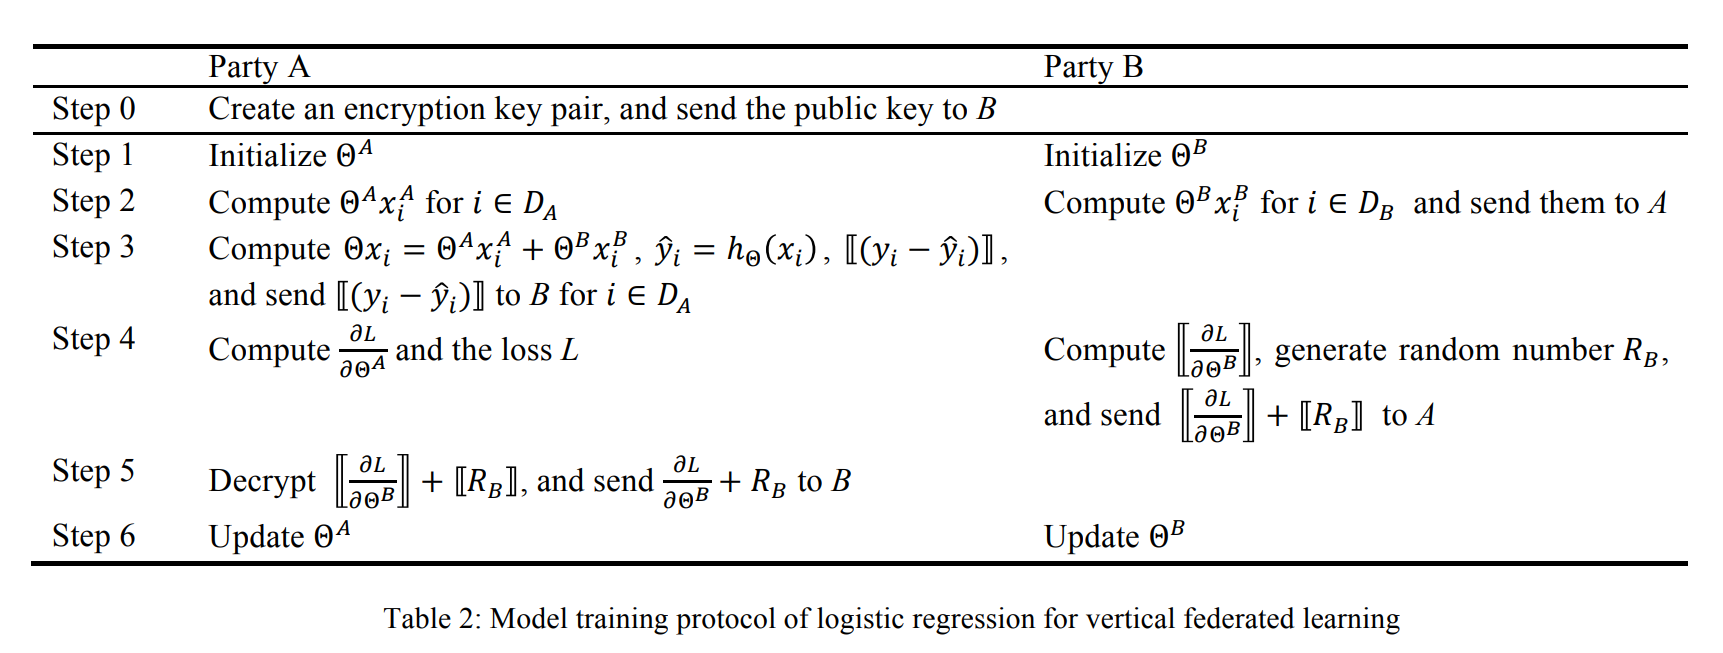
\includegraphics[width=0.8\textwidth]{pic/VFL-LR.png}
    \caption{VFL-LR算法主逻辑}
    \label{fig:VFL-LR}
\end{figure}

主逻辑的代码已经在附录中给出
其中大部分

\subsubsection{Accuracy计算}

\begin{lstlisting}
def _acc(self, y_true, y_hat):
    acc = np.mean(y_true == (y_hat >= 0.5))
    return acc
\end{lstlisting}

布尔数组与0,1数组在绝大多数情况下等价,布尔数组与0,1数组的比较、布尔数组的求平均值等操作中布尔数组的行为与0,1数组一致




\subsection{sacle函数的原理及作用}
% (20`)请说明代码中 scale 函数的原理及作用。



\subsection{随机数种子}
% (20`)当前代码在每个 epoch 开始时使用 epoch 值作为随机数种子,请说明含义,并实现另一种方式以达到相同的目的。

这是为了使得Party A\&B在每个epoch中使用相同的随机数,从而使得每次迭代中两边选择的样本下标一致,
从而可以将两边得到的label直接相加得到最终结果,也使得此结果可对正确下标的样本输入进行反向传播求导。


\section{实验结果}




\section{实验分析及开放题}
% (10`)开放题:试分析VFL-LR训练流程中潜在的隐私泄露风险,并简要说明可能的保护方式

\appendix
\section*{附录}

\section{Party A (Active Party)对一个batch进行处理的具体实现}

\begin{lstlisting}
total_loss = 0.0
total_acc = 0.0

for batch in range(n_batches):
    # Choose batch indexes
    start = batch * bs
    end = len(all_idxes) if batch == n_batches - 1 else (batch + 1) * bs
    batch_idxes = all_idxes[start:end]

    # Q1. Active party calculates y_hat
    # -----------------------------------------------------------------
    # self.params: (n_features, )
    # self.x_train[batch_idxes]: (batch_size, n_features)
    active_wx = np.dot(self.x_train[batch_idxes], self.params)  # (填空)计算A的wx
    passive_wx = self.messenger.recv()
    full_wx = active_wx + passive_wx  # (填空)综合A、B的wx(纵向联邦综合结果的关键一步)
    y_hat = self.activation(full_wx)
    # -----------------------------------------------------------------

    loss = self._loss(self.y_train[batch_idxes], y_hat)
    acc = self._acc(self.y_train[batch_idxes], y_hat)
    tbar.set_description(f"[loss={loss:.4f}, acc={acc:.4f}]")
    total_acc += acc * len(batch_idxes)
    total_loss += loss * len(batch_idxes)

    residue = self.y_train[batch_idxes] - y_hat
    residue = np.array([round(res, self.RESIDUE_PRECISION) for res in residue])

    # Q2. Active party helps passive party to calculate gradient
    # -----------------------------------------------------------------
    enc_residue = self.cryptosystem.encrypt_vector(residue)  # (填空)对误差进行加密
    enc_residue = np.array(enc_residue)
    self.messenger.send(enc_residue)

    enc_passive_grad = self.messenger.recv()
    passive_grad = self.cryptosystem.decrypt_vector(enc_passive_grad)  # (填空)解密得到B的梯度与梯度之和
    self.messenger.send(passive_grad)
    # -----------------------------------------------------------------

    # Active party calculates its own gradient and update model
    active_grad = self._gradient(residue, batch_idxes)
    self._gradient_descent(self.params, active_grad)
\end{lstlisting}

\section{Party B (Passive Party)对一个batch进行处理的具体实现}

\begin{lstlisting}
for batch in range(n_batches):
    # Choose batch indexes
    start = batch * bs
    end = len(all_idxes) if batch == n_batches - 1 else (batch + 1) * bs
    batch_idxes = all_idxes[start:end]

    # Q1. Calculate wx and send it to active party
    # -----------------------------------------------------------------
    passive_wx = np.dot(self.x_train[batch_idxes], self.params)  # (填空)计算B的预测值
    self.messenger.send(passive_wx)
    # -----------------------------------------------------------------

    # Q2. Receive encrypted residue and calculate masked encrypted gradients
    # -----------------------------------------------------------------
    enc_residue = self.messenger.recv()
    # print("enc_residue: ", enc_residue)
    enc_grad = self._gradient(enc_residue, batch_idxes)
    # print("enc_grad: ", enc_grad)
    enc_mask_grad, mask = self._mask_grad(enc_grad)
    self.messenger.send(enc_mask_grad)
    # Receive decrypted masked gradient and update model
    mask_grad = self.messenger.recv()
    true_grad = self._unmask_grad(mask_grad, mask)
    # -----------------------------------------------------------------

    self._gradient_descent(self.params, true_grad)
\end{lstlisting}

\end{document}
